%&fmt.out/fmt

\begin{document}
%    \includeonlyframes{current}

    \title{Автоматическое обнаружение гонок при параллельной сборке с использованием утилиты Make}
    \subtitle{}
    \date{20 июня 2024 г.}
    \author{Студент: Артем Климов \\ Научный руководитель: Дмитрий Мельник \\ Научные консультанты: Владислав Иванишин, Александр Монаков}
    \institute{\!
\includegraphics[width=10em]{logo_RU_basic.png}}

    \captionsetup{font=footnotesize,labelformat=empty}

%% /usr/share/texlive/texmf-dist/tex/latex/beamertheme-metropolis/beamerinnerthememetropolis.sty
    \setbeamertemplate{title page}{
        \begin{minipage}[b][\paperheight]{\textwidth}
            \vspace*{1mm}
            \vfill%
            \ifx\inserttitle\@empty\else\usebeamertemplate*{title}\fi
            \ifx\insertsubtitle\@empty\else\usebeamertemplate*{subtitle}\fi
%%     \usebeamertemplate*{title separator}
            \ifx\beamer@shortauthor\@empty\else\usebeamertemplate*{author}\fi
            \ifx\insertdate\@empty\else\usebeamertemplate*{date}\fi
            \ifx\insertinstitute\@empty\else\usebeamertemplate*{institute}\fi
            \ifx\inserttitlegraphic\@empty\else\usebeamertemplate*{title graphic}\fi
            \vfill
            \vspace*{2mm}
        \end{minipage}
    }

    \begin{frame}[plain] % Don't show slide number on the title slide.
        \titlepage
        \note{
            Здравствуйте, уважаемая комиссия. Меня зовут Артем, темой моей дипломной работы является "Автоматическое обнаружение гонок в параллельных сборках на основе Make".
        }
    \end{frame}

    \begin{frame}{План презентации}
        \begin{itemize}
            \setlength\itemsep{1.1em}
            \item \textbf{Введение}. Состояния гонок в Makefile. Примеры и формулировка проблемы.
            \item \textbf{Обзор существующих решений}.
            \item \textbf{Демонстрация} разработанного инструмента в виде сантайзера для Make.
            \item \textbf{Тестирование} решения на реальных проектах, \textbf{сравнение} с существующими решениями. \textbf{Заключение}.
        \end{itemize}

        \note{
            В рамках этой работы была исследована проблема состояний гонок в схемах сборки и разработан инструмент, с помощью которого их можно значительно легче обнаруживать.
        }
    \end{frame}


    \section{Введение}

%    \begin{frame}{Введение: Состояния гонок}
%
%        \textbf{Состояние гонки}~--- ситуация, когда несколько потоков работают с одним и тем же ресурсом одновременно,
%        и результат выполнения программы зависит от порядка выполнения потоков.
%
%        \begin{itemize}
%            \item Одновременное чтение и запись по одному и тому же адресу;
%            \item Создание каталога и одновременная работа с его содержимым;
%            \item Удаление ресурса без ожидания окончания его использования.
%        \end{itemize}
%
%        \note{
%            Начну с определения состояния гонки. Это ситуация, когда несколько потоков одновременно работают с \textbf{одним}
%            ресурсом, и результат выполнения программы зависит от \textbf{порядка}, в котором они выполняются.
%        }
%
%    \end{frame}

    \begin{frame}{Введение: Состояния гонок}

        Пример: Два потока пытаются увеличить переменную \texttt{counter}, если она меньше 1.

        \lstinputlisting[language=C++]{src/racesample.cpp}

        С неудачным планированием переменная может быть увеличена дважды, и окончательное значение будет равно 2.

        \note{
            Обычно о состояниях гонок говорят в контексте языков программирования, таких как C++ или Java. В них гонки могут возникать из-за недостаточной синхронизации между процессами. Например, из-за забытого мьютекса, как в примере на экране.
        }

    \end{frame}

    \begin{frame}{Введение: Состояния гонки в схемах сборки}
        \begin{itemize}
            \item Цели сборки могут собираться параллельно;
            \item При отсутствии необходимой синхронизации могут возникать гонки.
        \end{itemize}

        \begin{center}
            \begin{tikzpicture}
                \node[style=draw, minimum width=1.5cm] (libcpp) at (2,1.5) {lib.cpp};
                \node[style=draw, minimum width=1.5cm] (libo) at (4,1.5) {lib.o};
                \node[style=draw, minimum width=1.5cm] (liba) at (6,1.5) {lib.a};

                \node[style=draw, minimum width=3cm] (appcpp) at (2.75,0) {app.cpp};
                \node[style=draw, minimum width=3cm] (appo) at (6.25,0) {app.o};
                \node[style=draw, minimum width=3cm] (app) at (9.75,0) {app};

                \node[text width=5cm] at (10.5,1.1) {
                    \texttt{app} зависит от \texttt{lib.a}, но \textbf{не дожидается его сборки}
                };

                % liba -> app
                \draw[gray, dashed, line width=1pt, shorten >=2pt, shorten <=2pt, ->]
                (liba) to[out=0, in=180] ($(app.west) + (0, 0.12)$);

                % Common
                \node[minimum width=16cm, minimum height=3.5cm] (sizer) at (6.5,0.3) {};
                \node at (0,1.5) {Поток 1:};
                \node at (0,0) {Поток 2:};

                % appo -> app
                \draw[line width=1pt, shorten >=2pt, shorten <=2pt, ->]
                ($(appo.east) + (0,-0.12)$) -- ($(app.west) + (0,-0.12)$);

                % Time text and arrow
                \node[font=\itshape] (time) at (11.4, -1.16) {$\tau$};
                \draw[line width=0.7pt, ->] (0, -1.16) to (11, -1.16);

                \draw[line width=1pt, shorten >=2pt, shorten <=2pt, ->] (libcpp) -- (libo);
                \draw[line width=1pt, shorten >=2pt, shorten <=2pt, ->] (libo) -- (liba);
                \draw[line width=1pt, shorten >=2pt, shorten <=2pt, ->] (appcpp) -- (appo);
            \end{tikzpicture}
        \end{center}

        \note{
            Сборка программных проектов тоже может производиться многопоточно. Там, вместо мьютексов, семафоров или условных переменных примитивами синхронизации являются зависимости между целями сборки. Отсутствие нужной зависимости, по аналогии с отсутствием мьютекса в предыдущем слайде, может привести к состоянию гонки.

            На слайде изображен процесс сборки некоторого проекта. В нём приложение может собираться параллельно с библиотекой, которую оно использует. В этой схеме не хватает одной зависимости, которая бы задерживала компоновку приложения до момента, когда библиотека будет собрана.
        }
    \end{frame}

    \begin{frame}{Введение: Состояния гонки в схемах сборки}
        \begin{itemize}
            \item Если сборка библиотеки затянется, произойдет ошибка:
        \end{itemize}

        \begin{center}
            \begin{tikzpicture}
                \node[style=draw, minimum width=2.2cm] (libcpp) at (2.35,1.5) {lib.cpp};
                \node[style=draw, minimum width=2.2cm] (libo) at (5.2,1.5) {lib.o};
                \node[style=draw, minimum width=2.2cm] (liba) at (8.05,1.5) {lib.a};

                \node[style=draw, minimum width=2cm] (appcpp) at (2.25,0) {app.cpp};
                \node[style=draw, minimum width=2cm] (appo) at (4.75,0) {app.o};
                \node[style=draw, minimum width=2cm] (app) at (7.25,0) {app};
                \node[red, style=draw, minimum width=2cm] (ошибка) at (9.75,0) {ошибка};

                \node[red, style=draw, dashed, minimum width=4cm] (error) at (3.5,0.75) {lib.a еще не готова};

                \draw[red, dashed, line width=1pt, shorten >=2pt, shorten <=2pt, ->]
                (error) to[out=0, in=180] ($(app.west) + (0, 0.12)$);

                \draw[red, line width=1pt, shorten >=2pt, shorten <=2pt, ->] (app) -- (ошибка);

                % Common
                \node[minimum width=16cm, minimum height=3.5cm] (sizer) at (6.5,0.3) {};
                \node at (0,1.5) {Поток 1:};
                \node at (0,0) {Поток 2:};

                % appo -> app
                \draw[line width=1pt, shorten >=2pt, shorten <=2pt, ->]
                ($(appo.east) + (0,-0.12)$) -- ($(app.west) + (0,-0.12)$);

                % Time text and arrow
                \node[font=\itshape] (time) at (11.4, -1.16) {$\tau$};
                \draw[line width=0.7pt, ->] (0, -1.16) to (11, -1.16);

                \draw[line width=1pt, shorten >=2pt, shorten <=2pt, ->] (libcpp) -- (libo);
                \draw[line width=1pt, shorten >=2pt, shorten <=2pt, ->] (libo) -- (liba);
                \draw[line width=1pt, shorten >=2pt, shorten <=2pt, ->] (appcpp) -- (appo);
            \end{tikzpicture}
        \end{center}

        \note{
            Из-за этой забытой зависимости успешность сборки будет зависеть от того, успеет ли библиотека собраться раньше, чем будет запущен компоновщик. Если разработчику не повезёт и сборка библиотеки займёт много времени, то сборка всего проекта может завершиться неудачей.
        }
    \end{frame}

    \begin{frame}{Введение: Состояния гонки в схемах сборки}
        \begin{itemize}
            \item \textbf{Решение:} Определить пропущенную зависимость и добавить ее в схему сборки.
        \end{itemize}

        \begin{center}
            \begin{tikzpicture}
                \node[style=draw, minimum width=2.2cm] (libcpp) at (2.35,1.5) {lib.cpp};
                \node[style=draw, minimum width=2.2cm] (libo) at (5.2,1.5) {lib.o};
                \node[style=draw, minimum width=2.2cm] (liba) at (8.05,1.5) {lib.a};

                \node[style=draw, minimum width=2cm] (appcpp) at (2.25,0) {app.cpp};
                \node[style=draw, minimum width=2cm] (appo) at (4.75,0) {app.o};
                \node[style=draw, minimum width=2cm] (app) at (10.8,0) {app};

                \node[text width=3.6cm] at (8,0.5) {
                    \small{Поток 2 ждёт \texttt{lib.a} перед сборкой \texttt{app}}
                };

                % liba -> app
                \draw[line width=1pt, shorten >=2pt, shorten <=2pt, ->]
                (liba) to[out=0, in=180] ($(app.west) + (0, 0.12)$);

                % Common
                \node[minimum width=16cm, minimum height=3.5cm] (sizer) at (6.5,0.3) {};
                \node at (0,1.5) {Поток 1:};
                \node at (0,0) {Поток 2:};

                % appo -> app
                \draw[line width=1pt, shorten >=2pt, shorten <=2pt, ->]
                ($(appo.east) + (0,-0.12)$) -- ($(app.west) + (0,-0.12)$);

                % Time text and arrow
                \node[font=\itshape] (time) at (11.4, -1.16) {$\tau$};
                \draw[line width=0.7pt, ->] (0, -1.16) to (11, -1.16);

                \draw[line width=1pt, shorten >=2pt, shorten <=2pt, ->] (libcpp) -- (libo);
                \draw[line width=1pt, shorten >=2pt, shorten <=2pt, ->] (libo) -- (liba);
                \draw[line width=1pt, shorten >=2pt, shorten <=2pt, ->] (appcpp) -- (appo);
            \end{tikzpicture}
        \end{center}

        \note{
            Встретив такую ошибку, разработчик может либо попробовать ещё раз, либо разобраться в причине и добавить недостающую зависимость в схему, что устранило бы проблему.
        }
    \end{frame}

    \begin{frame}{Введение: Состояния гонок в реальных проектах}
        \tikz[remember picture, overlay] \node[text width=\textwidth, minimum width=\textwidth] at ($(current page.center)-(0,-2.5)$) {
            Ошибки сборки, связанные с состояниями гонок, часто становятся предметом обсуждения на форумах:
        };

        \tikz[remember picture, overlay] \node[anchor=center] at ($(current page.center)-(0,-0.5)$) {
            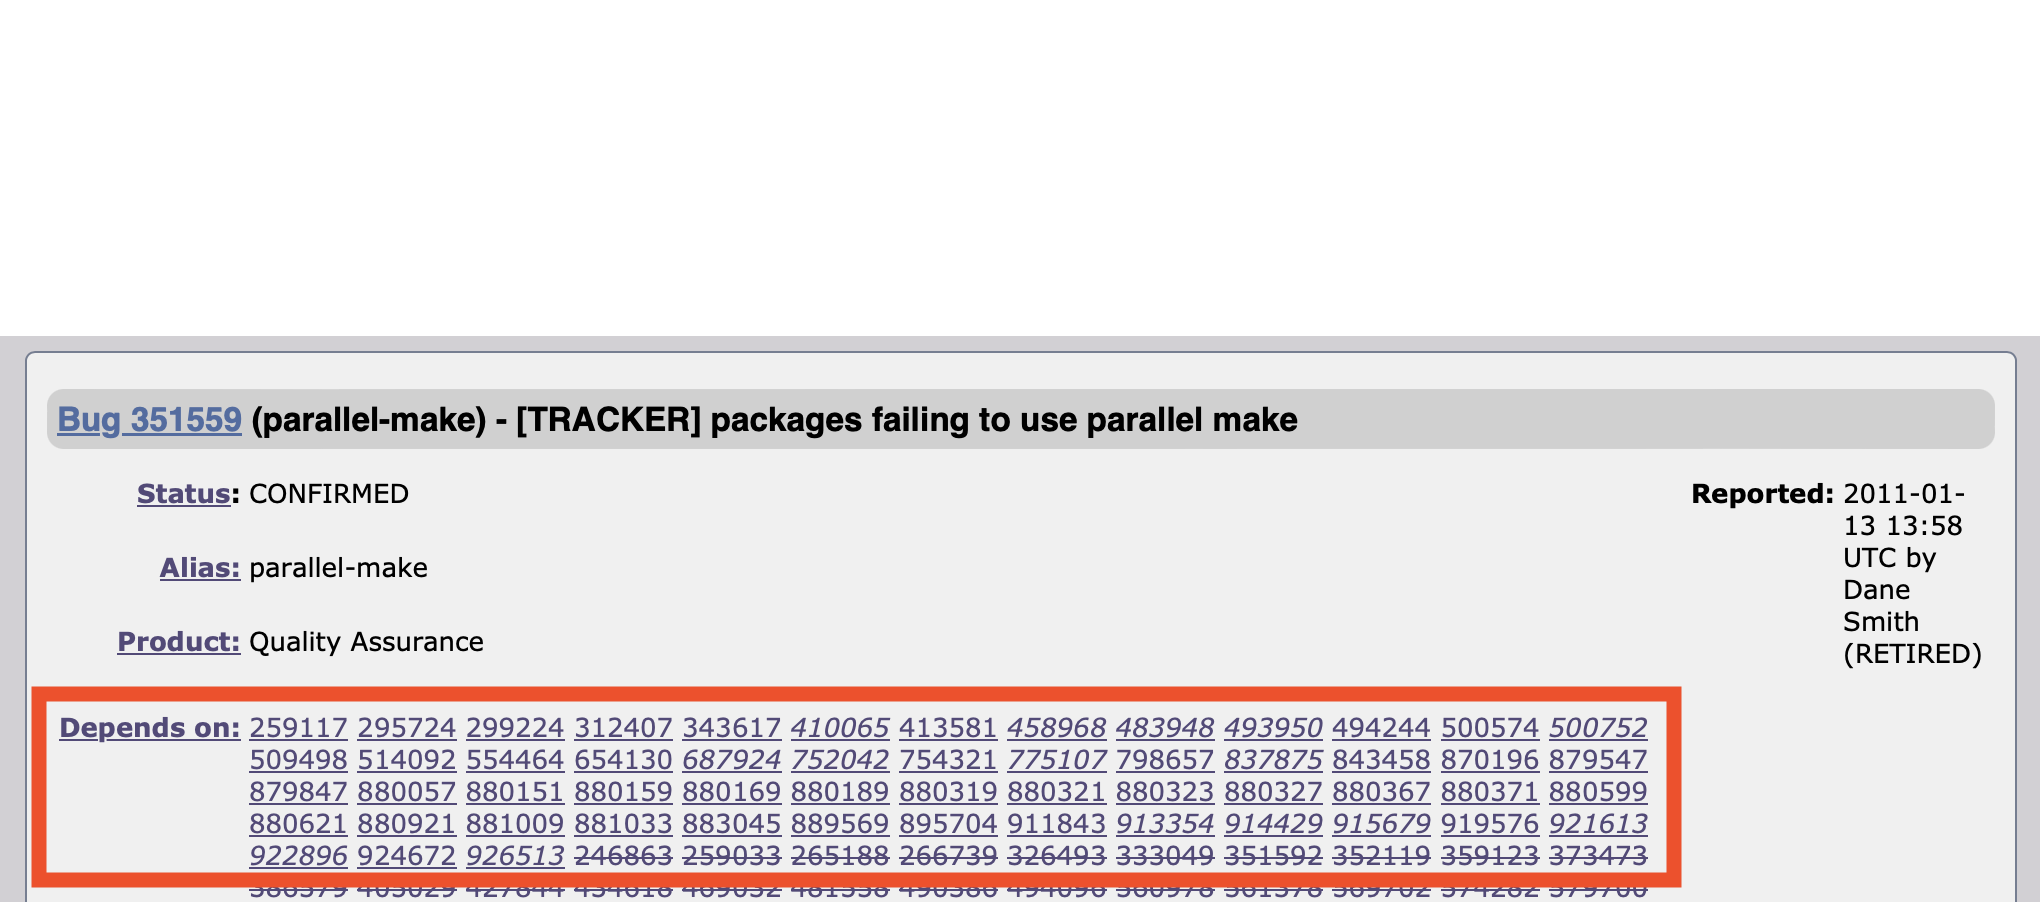
\includegraphics[width=1.1\textwidth]{gentoo-races}
        };

        \note{
            Состояния гонок часто проявляются как плавающие баги, которые трудно и редко воспроизводятся. В связи с этим, их сложно искать и отлаживать вручную. Подтверждение этому можно найти на форуме Gentoo, где в настоящее время открыто свыше 50 обсуждений на эту тему. Некоторые из них были открыты более 10 лет назад и по-прежнему остаются нерешенными.
        }
    \end{frame}

    \begin{frame}{Введение: Формулировка проблемы}

        Состояния гонок в схемах сборки являются актуальной проблемой:

        \begin{itemize}
            \item Сценарий гонки может редко воспроизводиться;
            \item Состояния гонок могут приводить не только к ошибкам сборки, но и к уязвимостям и проблемам в успешно собраннном проекте.
        \end{itemize}

        \textbf{Цель исследования:} Разработать инструмент для упрощения поиска и отладки состояний гонок в схемах сборки. Требования к нему:

        \begin{itemize}
            \item Обнаруживать все гонки, связанные с отсутствующими зависимостями;
            \item Выдавать детерминированный результат;
            \item Легко встраиваться в проекты;
            \item Не требовать \texttt{-j1} или многократных пересборок.
        \end{itemize}

        \note{
            Состояния гонок коварны тем, что являются скрытой проблемой, которая может проявиться самым нежелательным образом. Спонтанная ошибка сборки~--- даже не самое страшное ее проявление. Возможен сценарий, в котором состояния гонок могут привести к уязвимостям и другим проблемам в собранном проекте.

            Это подводит к \textbf{цели} работы: разработать инструмент, который позволял бы обнаруживать такие гонки автоматически. Основная его задача --- снизить время и усилия, необходимые для поиска и отладки гонок. Для этого он должен легко встраиваться в любые проекты и обнаруживать максимальное количество гонок за не более чем одну его пересборку.
        }
    \end{frame}


    \section{Обзор существующих решений}

    \begin{frame}{Обзор существующих решений: Bazel}
        \begin{itemize}
            \item Система сборки Bazel~--- использует песочницы для устранения случайности.
            \item Каждая цель собирается в своей песочнице.
            \item Каждая песочница имеет только файлы, собранные целями-зависимостями.
        \end{itemize}

        \begin{center}
            \begin{tikzpicture}
                \node[style=draw, rounded corners, inner xsep=7pt, inner ysep=7pt, align=center, minimum width=1.5cm, text width=1.5cm] (prereq1) at (0,0) {
                    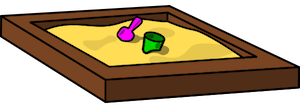
\includegraphics[width=1.5cm]{sandbox} \\
                    prereq1
                };
                \node[style=draw, rounded corners, inner xsep=7pt, inner ysep=7pt, align=center, minimum width=1.5cm, text width=1.5cm] (prereq2) at (0,-2) {
                    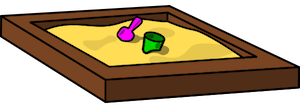
\includegraphics[width=1.5cm]{sandbox} \\
                    prereq2
                };
                \node[style=draw, rounded corners, inner xsep=7pt, inner ysep=7pt, align=center, minimum width=1.5cm, text width=1.5cm] (prereq3) at (10,0) {
                    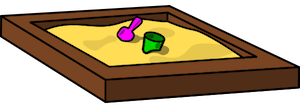
\includegraphics[width=1.5cm]{sandbox} \\
                    prereq3
                };
                \node[style=draw, rounded corners, inner xsep=7pt, inner ysep=7pt, align=center, minimum width=1.5cm, text width=1.5cm] (prereq4) at (10,-2) {
                    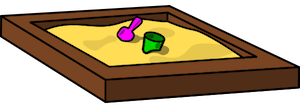
\includegraphics[width=1.5cm]{sandbox} \\
                    prereq4
                };

                \node[style=draw, rounded corners, inner xsep=7pt, inner ysep=7pt, align=center, minimum width=1.5cm, text width=1.5cm] (target) at (5,-1) {
                    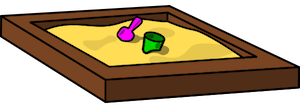
\includegraphics[width=1.5cm]{sandbox} \\
                    target
                };

                \draw[->, thick, shorten >=2pt, shorten <=2pt] (prereq1) to[out=0, in=180] (target);
                \draw[->, thick, shorten >=2pt, shorten <=2pt] (prereq2) to[out=0, in=180] (target);
                \draw[->, thick, shorten >=2pt, shorten <=2pt] (prereq3) to[out=180, in=0] (target);
                \draw[->, thick, shorten >=2pt, shorten <=2pt] (prereq4) to[out=180, in=0] (target);

                \node[rotate=-17] at (2.1, 0) {file1};
                \node[rotate=17] at (2.1, -2) {file2};
                \node[rotate=17] at (7.9, 0) {file3};
                \node[rotate=-17] at (7.9, -2) {file4};
            \end{tikzpicture}
        \end{center}

        \note{
            В современных системах сборки принимаются меры для борьбы с состояниями гонки. Например, Bazel позволяет производить сборку каждой цели в отдельной песочнице, в которой будут доступны только файлы, полученные в ходе сборки зависимостей. Это исключает гонки: с каждой такой виртуальной файловой системой работает одновременно лишь одна цель сборки, в определённом фиксированном порядке.
        }
    \end{frame}

    \begin{frame}{Обзор существующих решений: make -{}-shuffle}
        \begin{itemize}
            \item \texttt{make -{}-shuffle}~--- перемешивает список пререквизитов каждой цели.
            \item Это увеличивает вероятность проявления гонки, но помогает не всегда.
        \end{itemize}

        \vspace{0.5cm}

        \begin{center}
            \texttt{target: prereq1, prereq2, prereq3, ...}

            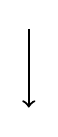
\begin{tikzpicture}
                \draw[->, thick] (0, 0) -- (0, -1);
            \end{tikzpicture}

            \texttt{target: prereq5, prereq2, prereq4, ...}
        \end{center}

        \note{
            Однако, Bazel и подобные системы пока не заменили собой классическую утилиту Make. Для неё существует только один известный мне инструмент, облегчающий поиск гонок. Это флаг \texttt{-{}-shuffle}, который позволяет случайным образом менять порядок сборки независимых целей, чтобы увеличить шанс проявления гонки. Однако, это требует полной пересборки проекта, может быть даже многократной. К тому же, как будет показано далее, многие гонки нельзя найти таким способом. Поэтому для дальнейшей работы выбрана именно система сборки Make.
        }
    \end{frame}


    \section{Реализация}

    \begin{frame}{Реализация: Архитектура}
        \begin{center}
            \begin{tikzpicture}
                \node[style=draw, rounded corners, inner xsep=10pt, minimum height=3cm] (trace) at (-1, -1) {Файл трассы};
                \node[style=draw, rounded corners, inner xsep=10pt, inner ysep=6pt] (tracer) at (3.2, 0) {Трассировщик};
                \node[style=draw, rounded corners, inner xsep=10pt, inner ysep=6pt] (make) at (7, 0) {remake*};
                \node[minimum width=2cm, minimum height=0.7cm, gray, style=draw, rounded corners] (child1) at (11, 1) {gcc};
                \node[minimum width=2cm, minimum height=0.7cm, gray, style=draw, rounded corners] (child2) at (11, 0) {mkdir};
                \node[minimum width=2cm, minimum height=0.7cm, gray, style=draw, rounded corners] (child3) at (11, -1) {...};

                \draw[dashed, gray, line width=1pt, shorten >=2pt, shorten <=2pt, ->] (tracer) -- (make);
                \draw[dashed, gray, line width=1pt, shorten >=2pt, shorten <=2pt, ->] (make) to[in=180, out=0] (child1);
                \draw[dashed, gray, line width=1pt, shorten >=2pt, shorten <=2pt, ->] (make) to[in=180, out=0] (child2);
                \draw[dashed, gray, line width=1pt, shorten >=2pt, shorten <=2pt, ->] (make) to[in=180, out=0] (child3);

                \draw[blue, line width=1pt, shorten <=2pt] (10, 0.75) arc (90:180:0.5);
                \draw[blue, line width=1pt, shorten <=2pt] (10, -0.25) arc (90:180:0.5);
                \draw[blue, line width=1pt] (9.5, 0.25) -- (9.5, -0.75) arc (0:-90:0.5);
                \draw[blue, line width=1pt] (7, -0.5) -- (7, -0.75) arc (0:-90:0.5);
                \draw[blue, line width=1pt, shorten <=2pt, ->] (10, -1.25) -- (4, -1.25) arc (270:180:0.5) -- (3.5, -0.5);
                \node[blue, font=\small] at (5.25, -1.0) {События ptrace};

                \draw[orange, line width=1pt, shorten >=2pt, shorten <=2pt, ->] (4.5, 0.5) arc (0:90:0.5) -- (-1, 1.0) arc (90:180:0.5);
                \node[orange, font=\small] at (1.8, 1.2) {События над файлами и процессами};

                \draw[black!50!green, line width=1pt, shorten >=2pt, shorten <=2pt, ->] (7.5, 0.5) -- (7.5, 1.0) arc (0:90:0.5) -- (-1.5, 1.5) arc (90:180:0.5) -- (-2.0, 0.5);
                \node[black!50!green, font=\small] at (3, 1.7) {Соответствие процессов целям и граф зависимостей};

                \node[minimum width=2cm, minimum height=0.7cm, style=draw, rounded corners] (user) at (9.7, -4.8) {Вывод};

                \node[align=center, minimum width=2cm, text width=2cm, minimum height=1.5cm, style=draw, rounded corners] (inode) at (2, -3.5) {Поиск гонок на inode};
                \node[align=center, minimum width=2cm, text width=2cm, minimum height=1.5cm, style=draw, rounded corners] (path) at (4.5, -3.50) {Поиск гонок на пути};
                \node[align=center, minimum width=2cm, text width=2cm, minimum height=1.5cm, style=draw, rounded corners] (dir) at (7, -3.5) {Поиск гонок на каталоге};

                % bottom horizontal line -> inode
                \draw[line width=1pt, shorten >=2pt] (2.5,-4.8) arc (270:180:0.5);

                % bottom horizontal line -> path
                \draw[line width=1pt, shorten >=2pt] (5,-4.8) arc (270:180:0.5);

                % bottom horizontal line -> dir
                \draw[line width=1pt, shorten >=2pt] (7.5,-4.8) arc (270:180:0.5);

                % bottom horizontal line
                \draw[line width=1pt, shorten >=2pt, ->] (2.5,-4.8) -- (8.5,-4.8);

                % top horizontal line -> inode
                \draw[line width=1pt, shorten >=2pt, ->] (1.5,-2.2) arc (90:0:0.5);

                % top horizontal line -> path
                \draw[line width=1pt, shorten >=2pt, ->] (4,-2.2) arc (90:0:0.5);

                % top horizontal line -> dir
                \draw[line width=1pt, shorten >=2pt, ->] (6.5,-2.2) arc (90:0:0.5);

                % top horizontal line
                \draw[line width=1pt, shorten <=2pt] (0.5,-2.2) -- (6.5,-2.2);

            \end{tikzpicture}
        \end{center}

        \note {
            \begin{itemize}
                \item На слайде изображена общая архитектура санитайзера. Основная идея в том, чтобы логировать всю необходимую для поиска гонок информацию в файл, а после запускать на нём некоторый анализатор, который и будет обнаруживать гонки.

                \item В этот файл поступает информация из нескольких источников:

                \item Прежде всего --- от трассировщика, который перехватывает и логирует системные вызовы, происходящие во время сборки. Это позволяет восстановить дерево процессов и установить, какие процессы работали с какими файлами.

                \item Анализаторы используют эту информацию, и соотносят эти доступы с графом зависимостей. Его тоже нужно откуда-то получить.

                \item Для этого пришлось модифицировать саму утилиту Make. Кроме графа зависимостей, она также сообщает о том, какие процессы были созданы какими целями.

                \item К слову, вместо обычного GNU Make была взята его вариация, которая называется remake. Как оказалось, её намного легче собирать из исходников чем оригинальную утилиту.

                \item Самих анализаторов три. Каждый из них ищет свой тип гонок.
            \end{itemize}
        }
    \end{frame}

    \begin{frame}{Реализация: Виды гонок}
        \centering
        \begin{tikzpicture}[
            group/.style={thick, decorate, decoration={calligraphic brace, amplitude=6pt, raise=10pt}},
            group text/.style={pos=0.5, xshift=-2cm, text width=2cm, align=right},
        ]

            \draw[gray, dashed] (0, 0) -- (0, -5.5);
            \draw[gray, dashed] (3, 0) -- (3, -5.5);
            \draw[gray, dashed] (6, 0) -- (6, -5.5);
            \draw[gray, dashed] (9, 0) -- (9, -5.5);

            \node[fill=white, draw, minimum width=2.5cm, minimum height=1cm] at (0, 0.1) {\keyword{read}};
            \node[fill=white, draw, minimum width=2.5cm, minimum height=1cm] at (3, 0.1) {\keyword{write}};
            \node[fill=white, draw, minimum width=2.5cm, minimum height=1cm] at (6, 0.1) {\keyword{unlink}};
            \node[fill=white, draw, minimum width=2.5cm, minimum height=1cm] at (9, 0.1) {\keyword{dir\_lookup}};

            \node[fill=white, thick, circle, draw, minimum width=0.5cm, minimum height=0.5cm] at (0, -1) {};
            \node[fill=white, thick, circle, draw, minimum width=0.5cm, minimum height=0.5cm] at (3, -1) {};

            \node[fill=white, thick, circle, draw, minimum width=0.5cm, minimum height=0.5cm] at (3, -2) {};

            \node[fill=white, thick, circle, draw, minimum width=0.5cm, minimum height=0.5cm] at (0, -3) {};
            \node[fill=white, thick, circle, draw, minimum width=0.5cm, minimum height=0.5cm] at (6, -3) {};

            \node[fill=white, thick, circle, draw, minimum width=0.5cm, minimum height=0.5cm] at (3, -4) {};
            \node[fill=white, thick, circle, draw, minimum width=0.5cm, minimum height=0.5cm] at (6, -4) {};

            \node[fill=white, thick, circle, draw, minimum width=0.5cm, minimum height=0.5cm] at (3, -5) {};
            \node[fill=white, thick, circle, draw, minimum width=0.5cm, minimum height=0.5cm] at (9, -5) {};

            \draw[thick, shorten >=10pt, shorten <=10pt, <->] (0, -1) -- (3, -1);
            \draw[thick, ->] (3.276, -1.824) arc (135:-135:0.25cm) -- (3.25, -2.16);
            \draw[thick, shorten >=10pt, shorten <=10pt, ->] (0, -3) -- (6, -3);
            \draw[thick, shorten >=10pt, shorten <=10pt, <->] (3, -4) -- (6, -4);
            \draw[thick, shorten >=10pt, shorten <=10pt, ->] (3, -5) -- (9, -5);

            \draw [group] (-1, -2.45) -- (-1, -0.55) node [group text] {Гонки на inode};
            \draw [group] (-1, -4.45) -- (-1, -2.55) node [group text] {Гонки на пути};
            \draw [group] (-1, -5.45) -- (-1, -4.55) node [group text] {Гонки на каталоге};

        \end{tikzpicture}

        \note {
            На схеме показано, какие именно гонки покрывают эти три анализатора. Они работают на четырех видах доступов --- чтение, запись, удаление и \keyword{dir\_lookup}, о котором я расскажу немного позже.

            \begin{itemize}
                \item Первые две строчки отражают самые очевидные гонки --- между чтением и записью и между двумя записями. Чтение и запись может производиться по разным путям, если у файла есть несколько жёстких ссылок. Поэтому вместо путей здесь используются номера inode. Именно они помогают уникально идентифицировать содержимое файла, на котором в действительности и происходит гонка.

                \item Следующие две строки связаны с операцией удаления. Разница в том, что удаление файла в первую очередь влияет на видимость файла по определённому пути, а не на его содержимое. Поэтому эти гонки привязаны к путям, не к номерам inode. Такие гонки могут возникать, если в двух независимых целях используется одно и то же имя для временного файла. Далее в этой работе будет рассмотрена гонка в Vim, которая происходит именно по такому сценарию.

                \item Последняя строка отражает гонку между созданием каталога (то есть \keyword{write}) и созданием файла внутри него. Сложность в том, что директория и файл в ней это разные сущности, с разными путями и с разными номерами inode. Поэтому для поиска таких гонок используется тот самый \keyword{dir\_lookup}. Это искусственный вид доступа, который добавляется санитайзером вручную, когда в директории создаётся какой-либо файл.
            \end{itemize}
        }
    \end{frame}

    \begin{frame}{Реализация: Перехват системных вызовов}
        \begin{center}
            \renewcommand{\arraystretch}{1.5}
            \begin{tabular}{>{\raggedright\arraybackslash}m{3cm}>{\raggedright\arraybackslash}m{6cm}}
                \toprule
                \multicolumn{1}{c}{\textbf{Cистемный вызов}} & \multicolumn{1}{c}{\textbf{Cобытие для санитайзера}} \\
                \midrule
                \texttt{open(at)(at2)}                       & \keyword{read} или \keyword{write}                   \\
                \texttt{mkdir(at)}                           & \keyword{write}                                      \\
                \texttt{creat}                               & \keyword{write}                                      \\
                \texttt{rmdir}                               & \keyword{unlink}                                     \\
                \texttt{unlink(at)}                          & \keyword{unlink}                                     \\
                \texttt{rename(at)(at2)}                     & \keyword{unlink} целевого пути, если он существует.  \\
                \bottomrule
            \end{tabular}
        \end{center}
        \begin{itemize}
            \item Дополнительно отслеживается \texttt{fork}, \texttt{clone}, \texttt{exec}, \texttt{spawn}.
            \item Остальные системные вызовы фильтруются через \texttt{seccomp BPF}.
        \end{itemize}

        \note {
            В этом слайде перечислены системные вызовы, которые перехватываются монитором \texttt{ptrace}, и события для санитайзера, в которые они конвертируются. Большинство из них относятся к файловой системе. Остальные касаются создания новых процессов.

            Для фильтрации ненужных системных вызовов ядра используется \textbf{Berkeley Packet Filter} (BPF). Он позволяет эффективно фильтровать системные вызовы на уровне ядра, не уведомляя о них монитор \texttt{ptrace}. Это существенно снижает накладные расходы на перехват системных вызовов и ускоряет работу санитайзера.
        }
    \end{frame}

    \begin{frame}{Реализация: Метод критических доступов}
        \begin{itemize}
            \item Санитайзер сообщает о гонке путём поиска зависимостей между парами конфликтующих доступов;
            \item Разработан метод, позволяющий пропускать ненужные проверки, сокращая сложность до линейной.
        \end{itemize}

        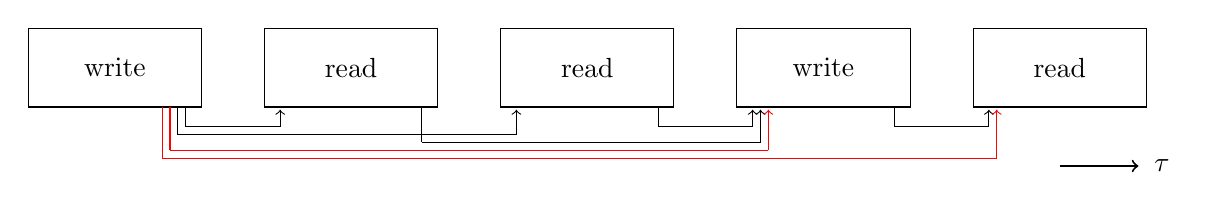
\begin{tikzpicture}
            \node[style=draw, minimum width=2.2cm, minimum height=1cm] at (0, -0.25) {write};
            \node[style=draw, minimum width=2.2cm, minimum height=1cm] at (3, -0.25) {read};
            \node[style=draw, minimum width=2.2cm, minimum height=1cm] at (6, -0.25) {read};
            \node[style=draw, minimum width=2.2cm, minimum height=1cm] at (9, -0.25) {write};
            \node[style=draw, minimum width=2.2cm, minimum height=1cm] at (12, -0.25) {read};

            % 0-1
            \draw (0.9,-0.75) -- (0.9,-1);
            \draw (0.9,-1) -- (2.1,-1);
            \draw[->, shorten >=1pt] (2.1,-1) -- (2.1,-0.75);

            % 2-3
            \draw (6.9,-0.75) -- (6.9,-1);
            \draw (6.9,-1) -- (8.1,-1);
            \draw[->, shorten >=1pt] (8.1,-1) -- (8.1,-0.75);

            % 4-5
            \draw (9.9,-0.75) -- (9.9,-1);
            \draw (9.9,-1) -- (11.1,-1);
            \draw[->, shorten >=1pt] (11.1,-1) -- (11.1,-0.75);

            % 0-2
            \draw (0.8,-0.75) -- (0.8,-1.1);
            \draw (0.8,-1.1) -- (5.1,-1.1);
            \draw[->, shorten >=1pt] (5.1,-1.1) -- (5.1,-0.75);

            % 1-3
            \draw (3.9,-0.75) -- (3.9,-1.2);
            \draw (3.9,-1.2) -- (8.2,-1.2);
            \draw[->, shorten >=1pt] (8.2,-1.2) -- (8.2,-0.75);

            % 0-3
            \draw[red] (0.7,-0.75) -- (0.7,-1.3);
            \draw[red] (0.7,-1.3) -- (8.3,-1.3);
            \draw[red, ->, shorten >=1pt] (8.3,-1.3) -- (8.3,-0.75);

            % 0-4
            \draw[red] (0.6,-0.75) -- (0.6,-1.4);
            \draw[red] (0.6,-1.4) -- (11.2,-1.4);
            \draw[red, ->, shorten >=1pt] (11.2,-1.4) -- (11.2,-0.75);

            \node[font=\itshape] (time) at (13.3, -1.5) {$\tau$};
            \draw[line width=0.7pt, ->] (12, -1.5) to (13, -1.5);
        \end{tikzpicture}

        \begin{itemize}
            \item Это позволяет санитайзеру работать быстро на проектах любого размера.
        \end{itemize}

        \note {
            Для поиска гонок санитайзер рассматривает пары конфликтующих доступов, и проверяет, что цели, которые их произвели, связаны зависимостью. Здесь возникает проблема: если проверять все возможные пары доступов, сложность алгоритма будет квадратичной. Это не позволит использовать санитайзер на больших проектах. Поэтому был разработан метод, который позволяет перебирать лишь минимальное, не более чем линейное необходимое множество пар, при этом гарантируя обнаружение любой возможной гонки. Этот метод был назван методом критических доступов.
        }
    \end{frame}

    \begin{frame}{Реализация: Особенности реализации}
        \begin{enumerate}
            \item Фильтр BPF и метод критических доступов увеличивает скорость работы санитайзера;
            \item Санитайзер поддерживает три вида гонок, полагается на номера inode, чтобы находить гонки между жёсткими ссылками;
            \item Санитайзер поддерживает установку точек останова и отладку с помощью интерактивной консоли;
            \item Отладка всех обнаруженных состояний гонок может производиться на одной и той же записанной трассе, без пересборки проекта.
        \end{enumerate}

        \note {
            Кратко перечислю основные особенности разработанного инструмента:

            \begin{itemize}
                \item Как я уже говорил, санитайзер работает быстро, использует разработанный нами метод критических доступов и BPF для фильтрации системных вызовов;
                \item Санитайзер может обнаруживать три разные категории гонок и использует номера inode, чтобы не пропускать гонки с жёсткими ссылками;
                \item Важным преимуществом, которое я не упоминал, является то, что санитайзер может выступать полноценным отладчиком. Он позволяет устанавливать точки останова на определённых доступах к файлам и просматривать состояние сборки в замороженном состоянии. При этом, чтобы начать отладку заново, не нужно пересобирать проект второй раз. Достаточно лишь запустить тот же файл трассы с начала. Это значительно ускоряет отладку.
            \end{itemize}
        }
    \end{frame}


    \section{Тестирование}

    \begin{frame}{Тестирование: Список проектов}
        Сергей Трофимович с помощью \texttt{make -{}-shuffle} обнаружил состояния гонок в 29 проектах с открытым исходным кодом, включая:

        \begin{enumerate}
            \item Vim
            \item GCC
            \item strace
            \item Ispell
        \end{enumerate}

        \url{https://trofi.github.io/posts/249-an-update-on-make-shuffle.html}

        \note {
            Для тестирования был использован список проектов, в которых были найдены гонки с помощью \texttt{make -{}-shuffle}.

            Список проектов был повзаимствован с блога Сергея Трофимовича, который, кстати, является разработчиком этого режима.

            В этом списке было 29 проектов, включая даже такие большие проекты, как GCC и Vim. Мы запустили наш санитайзер на каждом из них и проверили, что он находит те же гонки, что и \texttt{make -{}-shuffle}.
        }
    \end{frame}

    \begin{frame}{Тестирование: Vim}
        \begin{itemize}
            \item Ошибка при сборке Vim:
            \lstinputlisting[
                basicstyle=\small\ttfamily
            ]{src/vim-race.txt}
            \item \texttt{bin/vimtutor} не существует, хотя требуется целью \keyword{installtutorbin}.
            \item Санитайзер сообщил об этой гонке:
            \lstinputlisting[
                language=bash,
                alsoletter={/, _},
                escapechar=\%,
                numbers=none,
                morekeywords={inst\_dir/bin, installtutorbin, write, dir\_lookup}]
            {src/vim-reports.txt}
            \item Цели \keyword{inst\_dir/bin} и \keyword{installtutorbin} являются \textbf{неупорядоченными}
        \end{itemize}

        \note {
            Рассмотрим подробно одну из гонок в проекте Vim. Если обратиться к тексту ошибки, то можно предположить, что какой-то каталог создается слишком поздно, и цель \texttt{installtutorbin} не может обратиться к нему.

            Санитайзер, в свою очередь, нашел за нас \textbf{цель}, которая создает эту директорию, и определил, что она никак не зависит от цели, упомянутой в тексте ошибки. И как только это происходит, он сообщает, что это~--- действительно гонка, и согласно нашей классификации, это гонка на каталоге.

            Таким образом, мы автоматически нашли ту же гонку, которую прежде нашел живой человек, используя \texttt{make -{}-shuffle}
        }
    \end{frame}

    \begin{frame}{Тестирование: Другие гонки в Vim}
        \begin{itemize}
            \item Санитайзер также сообщил о ранее неизвестных гонках:

            \lstinputlisting[
                language=bash,
                alsoletter={/, _, .},
                escapechar=\%,
                numbers=none,
                morekeywords={gvim.desktop, vim.desktop, write, unlink}]{src/vim-new-race-report.txt}
            \item \texttt{LINGUAS} --- временный файл, используемый в двух независимых целях.
            \lstinputlisting[
                language=bash,
                alsoletter={/, _, .},
                escapechar=\%,
                morekeywords={gvim.desktop, vim.desktop},
                firstnumber=216]{src/vim-new-race.make}
            \item Эту гонку нельзя обнаружить с помощью \texttt{make -{}-shuffle}
        \end{itemize}

        \note {
            Интересно, что это далеко не единственная гонка в проекте Vim, которую наш санитайзер нашел.

            Он также нашел гонку второй категории, то есть гонку на пути. Если обратиться к мейкфайлу, то можно увидеть, что файл \texttt{LINGUAS} используется в двух независимых целях как временный файл.

            Эта гонка могла бы привести к тому, что Vim собрался бы без ошибок, однако имел бы поврежденные файлы локализации.

            Стоит также сказать, что \texttt{make -{}-shuffle} не помог бы в обнаружении этой гонки, поскольку она проявляется не от изменения порядка выполнения целей, а наоборот --- при их одновременном запуске. И это является еще одним преимуществом нашего инструмента.
        }
    \end{frame}

    \begin{frame}{Тестирование: Результаты}
        \tikz[remember picture, overlay] \node[anchor=center] at ($(current page.center)-(0.5,1.8)$) {
            \includegraphics[width=1.2\textwidth]{races}
        };
        \note {
            Вот результаты тестирования. Из всех 29 проектов санитайзер нашел референсные гонки в 23 из них. Довольно часто он находил еще и дополнительные гонки, которые ранее не были известны. Они изображены светло-синим цветом. Тёмно-синим изображены гонки, которые нашёл и наш санитайзер, и make \texttt{--shuffle}.

            В остальных пяти проектах ожидаемые гонки не были обнаружены. Они отмечены коричневым. Это связано с разными причинами --- например, санитайзер пока не умеет находить гонку между созданием символической ссылки и доступом к ней. Однако работы по улучшению санитайзера продолжаются, и в будущем мы надеемся найти все гонки из этого списка.
        }
    \end{frame}

    \begin{frame}{Тестирование: Замедление}
        \begin{itemize}
            \item Санитайзер замедляет сборку проекта на 11--13\% вне зависимости от его размера.
        \end{itemize}

        \begin{tabular}{lD{:}{:}{-1}D{:}{:}{-1}D{.}{.}{-1}}
            \toprule
            Программа & \multicolumn{1}{c}{Время сборки} & \multicolumn{1}{c}{Время сборки с санитайзером} & \multicolumn{1}{c}{Замедление} \\
            \midrule
            vim       & 0:18,3                           & 0:20,7                                          & 13,1\%                         \\
            x264      & 0:29,6                           & 0:33,0                                          & 11,5\%                         \\
            exifprobe & 0:01,36                          & 0:01,53                                         & 12,6\%                         \\
            angsd     & 0:21,3                           & 0:23,8                                          & 11,7\%                         \\
            gcc       & 50:28,0                          & 60:53,5                                         & 20,6\%                         \\
            \bottomrule
        \end{tabular}

        \note {
            Замедление при сборке составляет от 12\% на простых проектах до 20\% на gcc, который содержит длинные цепочки зависимостей и множество вложенных библиотек.
        }
    \end{frame}

    \begin{frame}{Тестирование: Выводы}
        Разработанный инструмент продемонстрировал свою эффективность и помог достичь цели исследования. Он был назван \textbf{parmasan}~--- \textbf{Par}allel \textbf{ma}ke \textbf{san}itizer.
        \vspace{2em}

        \textbf{Дальнейшие улучшения:}
        \begin{itemize}
            \item Улучшение учета символических ссылок в алгоритме поиска гонок;
            \item Интеграция инструмента в системы непрерывной интеграции;
            \item Добавление поддержки системы сборки \textbf{Ninja};
            \item Поддержка внешних отладчиков.
        \end{itemize}

        \textbf{Репозитории:}
        \begin{itemize}
            \item \url{https://github.com/ispras/parmasan}
            \item \url{https://github.com/ispras/parmasan-remake}
        \end{itemize}

        \note {
            Итак, подведу итог. в этой работе была исследована проблема состояний гонок в мейкфайлах, и разработан инструмент, который смог автоматически найти большинство уже известных гонок, а так же множество новых, которые до текущего времени оставались незамеченными.

            Инструмент получил название \textbf{parmasan} как акроним от \textbf{Par}allel \textbf{ma}ke \textbf{san}itizer.

            В дальнейшем планируется добавить в санитайзер поиск гонок с участием символических ссылок, добавить поддержку внешних графических отладчиков, интегрировать санитайзер в системы непрерывной интеграции, и добавить поддержку других систем сборки, таких как Ninja.

            На этом мой доклад завершён, и я готов ответить на ваши вопросы.
        }
    \end{frame}

%    \begin{frame}[standout,plain]
%        \vfill Спасибо за внимание! \vfill
%    \end{frame}
\end{document}

% - project icons
